\chapter{Ewaluacja modeli}

\section{Nauka modeli}

\subsection{Dobór parametrów}

Proces nauki poszczególnych modeli rozpoczęto od zdefiniowania \textit{hiper-parametrów} \cite{probst2018tunability}. Są to parametry, których wartości są ustawione przed rozpoczęciem procesu uczenia się i definiują one zachowanie poszczególnych warstw modelu. Początkowe wartości tych parametrów zdefiniowano zgodnie z powszechnymi wartościami używanymi w podobnych architekturach oraz na podstawie załączonej literatury. Dalsze kroki polegały na dostosowaniu tych parametrów do osiągnięcia najlepszego wyniku. Dobrym sposobem na znalezienie optymalnego doboru parametrów są metody typu wyszukiwanie w siatce (ang. \textit{grid search}) oraz wyszukiwanie losowe (ang. \textit{random search}) \cite{liashchynskyi2019grid}. Polegają one na porównywaniu działania modelu z przyjętymi parametrami wybranymi z przestrzeni parametrów. Podjęto próby użycia tych metod, jednak ze względu na ograniczone zasoby obliczeniowe oraz długi czas przetwarzania ograniczono przestrzeń parametrów do minimum. Pozwoliło to na przeszukanie bardzo małego zbioru wartości co i tak dało satysfakcjonujące wyniki.

Dobrane wartości dla modeli jednowarstwowego LSTM \ref{section:one_lstm} oraz głębokiego LSTM \ref{section:deep_lstm} przedstawiono w tabeli \ref{tab:parametry_lstm}. Założenie użycia tych samych hiper-parametrów dla obu modeli było sprawdzenie wpływu głębokości (liczby warstw) modelu na wynik. Rozmiar LSTM dotyczy liczby komórek LSTM w jednej warstwie, dobór wartości 120 zależał od wielkości zbioru danych oraz od ograniczeń zasobowych. Parametr przerywania (ang. \textit{dropout}) użyty do przeciwdziałania przeuczania się modelu został wybrany z pośród dwóch wartości 0.2 oraz 0.5, okazało się że 0.2 ma lepszy wpływ na wynik. Rozmiar wektora słów dotyczy szerokości gęstej reprezentacji wektorowej każdego słowa, czym większa wartość tym więcej informacji przenoszonej przez te wektory, jednak ograniczenia zasobów pozwoliły na szerokość 100, gdzie maksymalna dostępna szerokość to 300. Pozostałe parametry dotyczą sposobu nauki modeli oraz szybkości i długości tego procesu, wartości te pozostały domyślne.

\begin{table}[t]
\fcmtcaption{Tabela prezentująca wybrane \textit{hiper-parametry} modeli korzystających z LSTM.}\label{tab:parametry_lstm}
\centering\footnotesize%
\begin{tabular}{l c}
\toprule
\textit{hiper-parametr} & wartość \\
\midrule
rozmiar LSTM   & 120 \\
wskaźnik uczenia się   & 0.003 \\
przerywanie (ang. \textit{dropout})   & 0.2 \\
liczba epok   & 100 \\
rozmiar wektora słów   & 100 \\
wielkość grupy (ang. \textit{batch}) & 200 \\
\bottomrule
\end{tabular}
\end{table}

\subsection{Przebieg nauki}

Do procesu nauki użyto platformę \textit{Colab}\footnote{\url{https://colab.research.google.com/}}, która umożliwia korzystanie z zasobów karty graficznej (GPU) umożliwiającej dużo wydajniejszy proces nauki modeli. Dla jednowarstwowego LSTM czas przetwarzania jednej epoki to około 9 sekund, a dla modelu głębokiego LSTM to 64 sekundy. Przy użyciu laptopa czasy te były prawie dziesięciokrotnie większe co uniemożliwiło by tak sprawne projektowanie i dostrajanie modeli.

Proces nauki rozpoczęto od podstawowego modelu jednowarstwowego LSTM. Po doborze hiper-parametrów związanych z architekturą modelu dobrane były odpowiednie wartości dla liczby epok oraz wskaźnika uczenia się. Zauważono że po dwudziestej epoce dokładność przekroczyła 90\%, a po setnej epoce poprawa wyników była na tyle niewielka że przerwano proces nauki. Ostateczne wyniki są przedstawione na wykresach \ref{rys:lstm_one_deep_comparison} przedstawiających przebieg nauki dla modeli jednowarstwowego LSTM oraz głębokiego LSTM. W początkowych etapach nauki wartości funkcji straty (ang. \textit{loss}) oraz dokładności (ang. \textit{accuracy}) były bardzo podobne, jednak po dziesiątej epoce widać przewagę modelu głębokiego LSTM oznaczonego kolorem pomarańczowym. Wynikać to może z dużo większej złożoności tego modelu oraz możliwości zapamiętania przez ten model większej liczby cech przechowywanych w tekście.

\begin{figure}[t]
\centering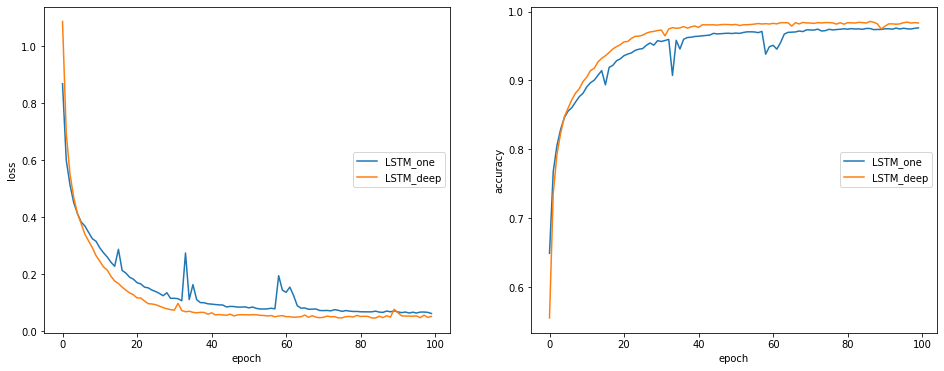
\includegraphics[width=\textwidth]{figures/reports/lstm_one_deep_comparison.png}
\fcmfcaption{Wykresy przedstawiające przebieg nauki dla modeli jednowarstwowego LSTM oraz głębokiego LSTM}\label{rys:lstm_one_deep_comparison}
\end{figure}

\section{Metryki}

\subsection{Macierz pomyłek}

W dziedzinie sieci neuronowych oraz oceny jakości modeli uczenia maszynowego, a w szczególności w problemach klasyfikacji często pomocna jest macierz pomyłek, inaczej nazywana macierzą błędów. Jest to specyficzny układ tabel, który pozwala na wizualizację wydajności algorytmu. Składa się on z dwóch wymiarów: rzeczywistym i przewidywanym. Podaje on liczbę wyników prawdziwie dodatnich (\textit{TP}), prawdziwie ujemnych (\textit{TN}), fałszywie dodatnich (\textit{FP}) oraz fałszywie ujemnych(\textit{FN}).

\begin{table}[ht]
\fcmtcaption{Tabela ukazująca macierz pomyłek.}\label{tab:tabela_matrix}
\centering\footnotesize%
\begin{tabular}{l|l|c|c|}
\multicolumn{2}{c}{}&\multicolumn{2}{c}{Prawdziwa etykieta}\\
\cline{3-4}
\multicolumn{2}{c|}{}&Positive&Negative\\
\cline{2-4}
\multirow{2}{*}{Przewidziana etykieta} & Positive & $TP$ & $FP$\\
\cline{2-4}
& Negative & $TN$ & $FN$\\
\cline{2-4}
\multicolumn{1}{c}{} & \multicolumn{1}{c}{Łącznie} & \multicolumn{1}{c}{$P$} & \multicolumn{1}{c}{$N$}\\
\end{tabular}
\end{table}

Pozwala to na bardziej szczegółową analizę oraz formułowanie wielu metryk na podstawie wartości z tej macierzy. Niektóre z tych miar zastosowano do ewaluacji modeli i zaprezentowano w kolejnych podsekcjach.

\subsection{Miara jakości nauki}

Główną metryką analizowaną w trakcie nauki modelu była dokładność (ang. \textit{accuracy}), zdefiniowana w poniższym równaniu \ref{eqn:accuracy}.

\begin{equation}
\label{eqn:accuracy}
dokladnosc=\frac{TP + TN}{P + N}
\end{equation}

Miara ta odwzorowuje efektywność nauki. Podczas jej obserwacji można stwierdzić czy każda kolejna epoka nauki poprawia wynik, czy też go pogarsza. Zbiór danych treningowy miał zrównoważony rozkład klas na tyle, że zastosowanie tej metryki miało sens. Niestety jeśli zestaw danych mocno niezbalansowany, tak jak w przypadku zbioru testowego miara ta może wprowadzić w błąd. Z tego powodu zastosowanie tej metryki ograniczono tylko do obserwacji procesu nauki, a ostateczną ocenę modelu wykonano na podstawie innych miar.

\subsection{Ostateczna ocena modelu}

Ostateczną ocenę modelu dokonano za pomocą obliczenia mikro średniego wyniku F1 dla trzech klas emocji \textit{Happy}, \textit{Sad}, \textit{Angry}. Wybór ten wynika z niezbalansowania klas w zbiorze testowym oraz dominacją występowania etykiety \textit{Others}, którą pominięto w ostatecznej ocenie. Wynik F1 jest średnią harmoniczną precyzji i czułości, zdefiniowanych w poniższych wzorach. Końcowy wynik uzyskany jest poprzez uśrednianie w skali mikro, na podstawie częstotliwości klas występujących w zbiorze treningowym. Poniższe wzory przedstawiają poszczególne składniki oraz samą funkcję F1.

\begin{equation}
\label{eqn:precyzja}
precyzja = \frac{TP}{FP+TP}
\end{equation}

\begin{equation}
\label{eqn:czułość}
czulosc = \frac{TP}{FP+TP}
\end{equation}

\begin{equation}
\label{eqn:f1}
F1 = \frac{2 \cdot precyzja\cdot czulosc}{precyzja + czulosc}
\end{equation}

\section{Wyniki}

Jakość wyuczonych modeli na zbiorze treningowym porównano poprzez ewaluację predykcji tych modeli na zbiorze testowym. Głównymi założeniami porównań było sprawdzenie wpływu liczby warstw sieci neuronowej na wynik oraz porównanie tradycyjnych rekurencyjnych warstw do bardziej złożonych architektur jakim jest BERT. 

Porównanie jednowarstwowej architektury LSTM  z głęboką architekturą LSTM pokazuje przewagę dla modelu głębokiego. Większa liczba warstw pomogła osiągnąć lepszy wynik miary mikro F1, jednak jest to niewielka poprawa. Można spekulować że jednowarstwowa sieć LSTM dla tego zbioru danych była wystarczająca aby osiągnąć maksimum możliwości tej architektury. Z drugiej strony użycie gęstej reprezentacji wektorowej każdego słowa mogło ograniczyć możliwości warstw LSTM i spowodować że użycie kolejnych warstw sieci pomogło na zniwelowanie tylko małych błędów. Niestety analiza wpływu na wynik poszczególnych elementów sieci neuronowej jest utrudniona co uniemożliwia wyciągnięcie jasnych i sprawdzonych wniosków.

TODO BERT

\begin{table}[ht]
\fcmtcaption{Tabela pokazująca wyniki poszczególnych modeli.}\label{tab:tabela_results}
\centering\footnotesize%
\begin{tabular}{c c c c c}
\toprule
model & dokładność & mikro precyzja & micro czułość & mikro F1 \\
\midrule
Jednowarstwowy LSTM   & 0.85 & 0.49 & 0.70 & 0.58 \\
Głęboki LSTM   & 0.87 & 0.51 & 0.71 & 0.60 \\
BERT todo   & xx & xx & xxx & xxx \\
\bottomrule
\end{tabular}
\end{table}